\chapter{Modification apportée au programme principale (DSP)}

\begin{enumerate}
    \item Machine Etat
    \item Conversion courant et pos modif par rapport a
    \item Structure et propeté du code
    \item correction de la pos
\end{enumerate}

\section{Introduction}
Suite au différentes modification réaliser sur le hardware ainsi que sur la régulation, le programme principale reçu dès lors d'importante modification. Ce chapitre vient traiter ces différences.

La mise en place de Code Composer Studio est disponible dans le manuel, à la \autoref{sec:MiseEnPlace}.

\section{Machine d'état}
Une machine d'état fut réaliser. Celui-ci doit pouvoir permettre de raéliser la régulation de position et de courant. Mais certaines étapes doivent être respecté afin de réussir cela.

Une première machine d'état fut réaliser présente dans les annexes (voir \ref{annexe:MachineEtatSISO})

Les étapes de la machine d'état sont les suivant :

\begin{itemize}
    \item Etat 0 : On attends la pression du boutton

    \item Etat 1 : On monte le courant des inducteurs 1\&2 à 3 A (pour ne pas partir de zéro).

    \item Etat 2 : On augmente le courant des inducteurs 1\&2 avec une rampe "infinie" (régulation de courant seule).

    \item Etat 3 : Lorsque l'inducteur 1\&2 commencent à bouger, on les passe en régulation de position SISO (lévitation de l'avant du véhicule).

    \item Etat 4 : On monte le courant des inducteurs 3\&4 à 3 A (pour ne pas partir de zéro).

    \item Etat 5 : On augmente le courant des inducteurs 3 et 4 avec une rampe "infinie" avec seulement le courant infinie, puis dès qu'un mouvement est détecté on passe imédiatement a la régulation MIMO

    \item Etat 6 : On attends d'éteindre la maquette.

    \item Etat 7 : On affiche un message d'erreur si la maquette rencontre un problème
\end{itemize}

Ceci est alors réalisé comme représenter dans la \autoref{fig:MachEtatMIMO} :

\begin{figure}[H]
    \centering
    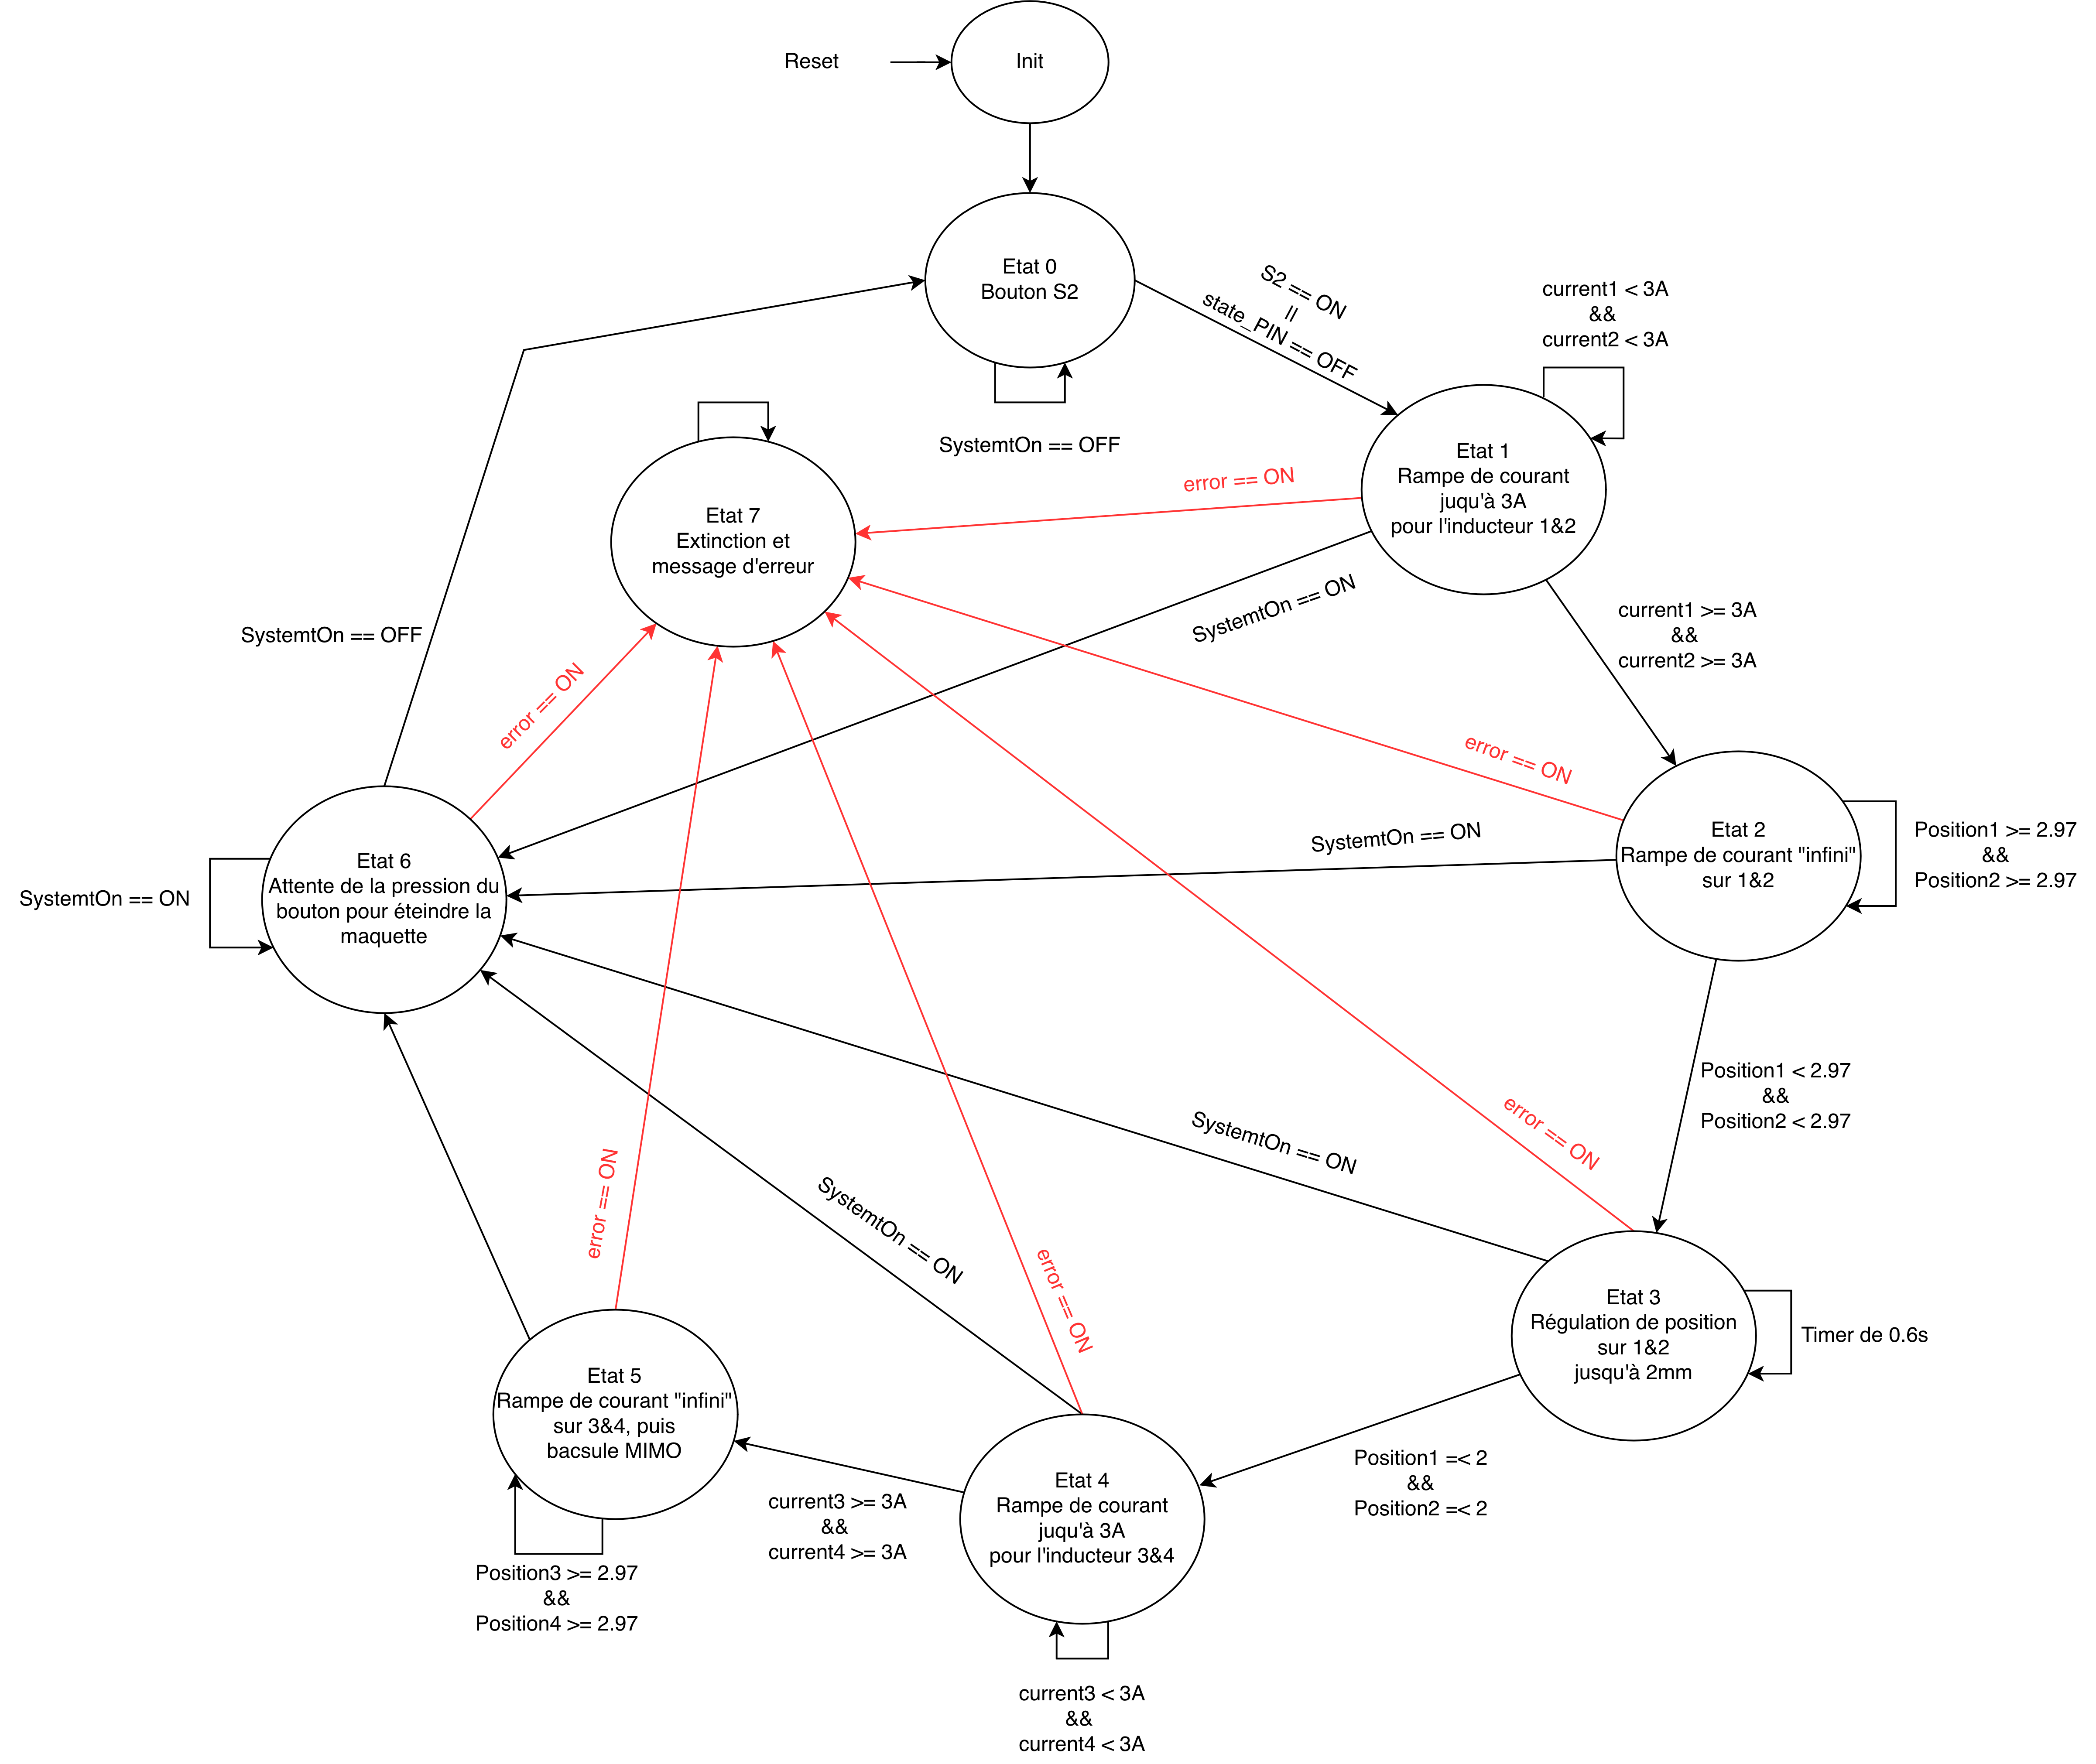
\includegraphics[width=1\linewidth]{assets/content/13-ModifDSP/MachineEtatMIMO.png}
    \caption{Machine d'état pour la régulation}
    \label{fig:MachEtatMIMO}
\end{figure}

Chaque état est dès lors implémenter dans le programme en suivant les étapes lister dessu..

L'état 0 est définit comme suit :

\begin{minted}{c}
    // State 0 :
    // Attente de la pression du bouton
    case STATE_0 :

        if(SystemOn)
        {
            GPIO_writePin(LED_D2, 0);

            state = SKIP_FRONT ? STATE_4 : STATE_1;
        }

    break;
\end{minted}

L'état 1 est implémenter comme cela :

\begin{minted}{c}
    // State 1 :
    // Rampe de courant sur les inducteurs 1&2 jusqu'a atteindre les 3A
    case STATE_1:

        if(ic1 < I_SP)
        {
            ic1 += TAKEOFF_CURRENT_STEP1;
        }
        else
        {
            ic1 = I_SP;
        }

        ic2 = ic1;

        mean1 += Current1;
        mean2 += Current2;
        dt_mean++;

        if(dt_mean >= 200)
        {
            mean1 = mean1 / dt_mean;
            mean2 = mean2 / dt_mean;

            if((mean1 <= I_SP105 && mean1 >= I_SP095) && (mean2 <= I_SP105 && mean2 >= I_SP095))
            {
                mean1 = 0;
                mean2 = 0;
                dt_mean = 0;

                state = STATE_2;
            }
            else
            {
                mean1 = 0;
                mean2 = 0;
                dt_mean = 0;
            }
        }

        break;
\end{minted}

L'état 2 est implémenter comme cela :

\begin{minted}{c}
    // State 2 :
    // Rampe de courant "infinie" jusqu'au decollage de l'avant
    case STATE_2:

        if(Position1 <= Position_c1_dec && Position2 <= Position_c2_dec)
        {
            Position_c1 = Position1;
            Position_c2 = Position2;

            xr1 = 0.0f;
            xr2 = 0.0f;
            pos_est1 = Position1; vit_est1 = 0.0f; for_est1 = 0.0f;
            pos_est2 = Position2; vit_est2 = 0.0f; for_est2 = 0.0f;

            state = STATE_3;
        }
        else if(ic1 < 9.5f)
        {
            ic1 += TAKEOFF_CURRENT_STEP1;
        }
        else
        {
            ic1 = 9.5f;
        }

        ic2 = ic1;

        break;
\end{minted}

L'état 3 est implémenter comme cela :

\begin{minted}{c}
    // State 3 :
    // Regulation SISO de l'avant, rampe de consigne 3mm -> 2mm
    case STATE_3:

        if(!PosRegFlag1) PosRegFlag1 = true;

        if(Position_c1 > DELTA_N)
        {
            Position_c1 -= 2.5 * 4e-7;
        }
        else
        {
            Position_c1 = DELTA_N;
        }

        if(Position_c2 > DELTA_N)
        {
            Position_c2 -= 2.5 * 4e-7;
        }
        else
        {
            Position_c2 = DELTA_N;
        }

        i_store++;

        if(i_store == I_STORE_2E_DECOLLAGE)
        {
            i_store = 0;

            state = SKIP_BACK ? STATE_7 : STATE_4;
        }

        break;
\end{minted}

L'état 4 est implémenter comme cela :

\begin{minted}{c}
    // State 4 :
    // Rampe de courant sur les inducteurs 3&4 jusqu'a atteindre les 3A
    case STATE_4:

        if(ic3 < I_SP)
        {
            ic3 += TAKEOFF_CURRENT_STEP1;
        }
        else
        {
            ic3 = I_SP;
        }

        ic4 = ic3;

        mean3 += Current3;
        mean4 += Current4;
        dt_mean++;

        if(dt_mean >= 200)
        {
            mean3 = mean3 / dt_mean;
            mean4 = mean4 / dt_mean;

            if((mean3 <= I_SP105 && mean3 >= I_SP095) && (mean4 <= I_SP105 && mean4 >= I_SP095))
            {
                mean3 = 0;
                mean4 = 0;
                dt_mean = 0;

                state = STATE_5;
            }
            else
            {
                mean3 = 0;
                mean4 = 0;
                dt_mean = 0;
            }
        }

        break;
\end{minted}

L'état 5 est implémenter comme cela \red{a modifier}:

\begin{minted}{c}
    // State 5 :
    // Rampe de courant "infinie" jusqu'au decollage de l'arriere,
    // puis bascule bumpless en regulation MIMO
    case STATE_5:

        if(Position3 <= Position_c3_dec && Position4 <= Position_c4_dec)
        {
            uint16_t j;
            float f_init0 = fc1f;
            float f_init1 = fc2f;
            float f_init2 = F_STAT[2];
            float f_init3 = F_STAT[3];

            for(j = 0; j < 3; j++)
            {
                float up = E_MAT[j][0]*f_init0 + E_MAT[j][1]*f_init1
                        + E_MAT[j][2]*f_init2 + E_MAT[j][3]*f_init3 - U_STAT[j];
                qm_ref[j] = qm[j];
                qm_est[j] = qm[j];
                vm_est[j] = 0.0f;
                um_est[j] = up;
                eps_m[j]  = -up * LQI_EPS_INV[j];
                u_cmd[j]  = up;
                u_sat[j]  = up;
                u_ach[j]  = up;
            }

            IN3[1] = F_STAT[2]; IN3[2] = F_STAT[2];
            OUT3[0] = F_STAT[2]; OUT3[1] = F_STAT[2];
            IN4[1] = F_STAT[3]; IN4[2] = F_STAT[3];
            OUT4[0] = F_STAT[3]; OUT4[1] = F_STAT[3];

            MimoFlag = true;

            state = STATE_6;
        }
        else if(ic3 < 9.5f)
        {
            ic3 += TAKEOFF_CURRENT_STEP1;
        }
        else
        {
            ic3 = 9.5f;
        }

        ic4 = ic3;


        break;
\end{minted}

L'état 6 est implémenter comme cela :

\begin{minted}{c}
    // State 6 :
    // Attend que le bouton soit presse a nouveau pour eteindre la maquette
    case STATE_6:

        if(!SystemOn)
        {
            uint16_t j;

            GPIO_writePin(LED_D2, 1);

            for(i = 0; i < NUM_OF_PWM_CHANNEL; i++)
            {
                dutyFine = ((float)(duty_cycle_table[i] * TIME_BASE_PERIOD) * INV_FACTOR);
                compCount = (dutyFine * (float32_t)(EPWM_TIMER_TBPRD << 8)) * INV_FACTOR;
                HRPWM_setCounterCompareValue(ePWM[i], HRPWM_COUNTER_COMPARE_A, compCount);
                HRPWM_setCounterCompareValue(ePWM[i], HRPWM_COUNTER_COMPARE_B, compCount);
            }

            PosRegFlag1 = false;
            MimoFlag = false;

            i_store = 0;

            integral_i1 = 0.0f; ue1 = 0.0f; ic1 = 0.0f;
            integral_i2 = 0.0f; ue2 = 0.0f; ic2 = 0.0f;
            integral_i3 = 0.0f; ue3 = 0.0f; ic3 = 0.0f;
            integral_i4 = 0.0f; ue4 = 0.0f; ic4 = 0.0f;

            xr1 = 0.0f; ep1 = 0.0f;
            xr2 = 0.0f; ep2 = 0.0f;

            for(j = 0; j < 3; j++)
            {
                eps_m[j] = 0.0f;
                u_cmd[j] = 0.0f;
                u_sat[j] = 0.0f;
                u_ach[j] = 0.0f;
                vm_est[j] = 0.0f;
                um_est[j] = 0.0f;
                qm_est[j] = qm[j];
                qm_ref[j] = qm_target[j];
            }

            status = SFO();
            if (status == SFO_ERROR) error();

            state = STATE_0;
        }

        break;
\end{minted}

\section{Régulation de position}
\subsection{Ajout des observateur}
\subsection{Régulation SISO}
\subsection{Régulation MIMO}

\section{Modifications mineures}
\subsection{Amélioration du code via l'IA}
Afin d'optimiser l'appropriation du code source hérité, une première révision syntaxique a été réalisée à l'aide d'outils d'intelligence artificielle. Cette démarche avait pour objectif d'améliorer la structure du programme, d'enrichir les commentaires et d'en accroître la lisibilité globale. Le comportement de la maquette a été rigoureusement contrôlé à la suite de cette restructuration purement formelle. Les résultats obtenus étant strictement identiques à ceux de la version d'origine, il est confirmé que cette intervention n'a introduit aucun dysfonctionnement supplémentaire.

\subsection{Création d'un fichier secondaire .c}
Ce fichier constitue une révision du travail initial mené par Thomas Freyche. Afin d'améliorer la clarté et la modularité du code source, les définitions ont été scindées sur deux fichiers distincts, bien que la logique de fonctionnement demeure strictement identique. Celle-i vient donc abriter les nombreuses fonctions du code.

\subsection{Modification des coefficients du filtre coupe-bande}
Toutefois, lors de l'analyse du code source hérité, il a été constaté que ces définitions n'étaient pas utilisées. Une autre variante de coefficients était active :

\begin{minted}{c}
//bandstop Filter 56Hz 2nd order bande coupe de 47Hz  90Hz (0) (test)
#define A1_B1_0         -1.980143772501098
#define A2_0            0.980339665209542
#define B0_B2_0         0.9901698326047711
\end{minted}

Cette disparité provient vraisemblablement d'essais expérimentaux antérieurs non documentés. Par souci de cohérence avec le travail de Laucella \cite{Laucella}, les paramètres ciblant la fréquence de 75~Hz ont été restaurés.

\subsection{Modification de l'emplacement du filtre coupe-bande}
Afin d'éviter un retard d'une période de 40~$\mu$s, le filtre a été placé juste après le calcul de la force. Précédemment, celui-ci se trouvait avant ce calcul et était employé pour le calcul de la consigne de courant.

\subsection{Modification de la variable d'enclenchement}



